\documentclass[TheoreticalPhy_ModB.tex]{subfiles}
\begin{document}

\chapter{Spontaneous Symmetry Breaking (SSB)}

Spontaneous symmetry breaking is one of the most important concepts in quantum field theory. The distinction between spontaneous and explicit symmetry breaking is that with spontaneous symmetry breaking the Lagrangian is invariant under the symmetry, but the ground state of the theory is not. With explicit symmetry breaking, there was never an exact symmetry to begin with. One usually associates spontaneous symmetry breaking with phase transitions. The amazing thing about spontaneous symmetry breaking is that one can say a tremendous amount about the broken phase with an effective theory whose input is the symmetry that was broken - no detailed microscopic description is needed. 

A simple example is given by a ferromagnet. The action governing its microscopic dynamic is invarian under spatial rotations. Above a critical temperature a ferromagnet has a unique ground state, with zero magnetization. Of course this state respects the rotational invariance, since on it the expectation value of the magentization $\vec M$ vanishes, and therefore no preferred direction is selected. Below a critical temperature instead it becomes thermodynamically favourable to develop a non-zero magnetization, and in this new vacuum $\vec M\neq0$ and the full $SO(3)$ rotational symmetry is broken to the subgroup $SO(2)$ of rotations around the magnetization axis. 

The original invariance of the Lagrangian is now reflected in the fact that, instead of a single vacuum state, there is a whole family of vacua related to each other by rotations, since the magnetization can in principle develop in any direction. However, the system will choose one of these states as its vacuum state. The symmetry is then said to be \emph{spontaneously broken} by the choice of a vacuum.

For $T<T_C$ it is helpful to write $\vec M(x)=\vec\mu+\vec\sigma(s)$, where $\vec\mu$ is the expectation value of $\vec M$ in the vacuum ($T=0$) and $\vec\sigma$ are the excitations around this minimum. The field $\vec\sigma(x)$ encodes spin waves whose quanta are called Goldstone bosons. 

For continuous global symmetry, such as $\phi(x)\to e^{i\alpha}\phi(x)$, the breaking of the symmetry automatically implies the existence of long-range correlations and associated massless particles. This is Goldstone's theorem, and the massless particles are called Goldstone bosons. If the symmetry is gauged, as for $\phi(x)\to\phi^{i\alpha(x)}\phi(x)$ with an associated massless gauge field $A_\mu(x)$, then in the broken phase the gauge boson will acquire a mass. This is known as the Higgs mechanism, and allows to describes Weak interactions (which are mediated throw massive bosons $W^\pm$ and $Z$) as a spontaneously broken (renormalizable) gauge theory (an explicit presence of a mass term in the Lagrangian broke the gauge symmetry, since any term in the form $M^2A_\mu A^\mu$ is not gauge invariant because of the transformation rule for gauge fields). 


\section{Spontaneous Symmetry Breaking of global symmetries}
\textsf{Maggiore sec. 11.1-11.2; Peskin sec. 11.1; Schwartz sec. 28.1-28.2; Mandl sec. 18.1; Halzen sec. 14.6-14.7}\\

\subsection{The renormalizable complex scalar potential and the sign of the quadratic term $\mu^2$}

The simplest example of a field theory exhibiting spontaneous symmetry breaking is the \emph{Goldstone model}, i.e. a complex scalar theory with $U(1)$ symmetry. The Lagrangian of this model is
\[\mathcal L=(\partial_\mu\phi^\dagger)(\partial^\mu\phi)-V(\phi^\dagger\phi)
\qquad \text{with}\qquad
V(\phi^\dagger\phi)=\lambda\left(\phi^\dagger\phi+\frac{\mu^2}2\right)^2
\]
This theory has a global $U(1)$ symmetry $\phi(x)\to e^{i\alpha}\phi(x)$ for constant $\alpha\in\mathR$. The Hamiltonian for this theory is
\[H=\int\de^3x\left\{|\pi|^2+|\vec\nabla\phi|^2+V(\phi^\dagger\phi)\right\}\]
hence we require $\lambda>0$ in such a way that the energy is bounded from below. We can see that no conditions is required for the parameter $\mu$, since in any case the potential is well defined. The Lagrangian can also be written in terms of two real fields $\phi_1$ and $\phi_2$ such that $\phi=(\phi_1+i\phi_2)/{\sqrt2}$:
\[\mathcal L=\frac12(\partial_\mu\phi_1)^2+\frac12(\partial_\mu\phi_2)^2-V(\phi_1^2+\phi_2^2)
\qquad \text{with}\qquad
V(\phi_1^2+\phi_2^2)=\frac\lambda4\left(\phi_1^2+\phi_2^2+\mu^2\right)^2
\]
In this representation the symmetry of the Lagrangian is $SO(2)\simeq U(1)$.

Let us discuss the proprieties of the ground state (vacuum) of the system. We define the vacuum expectation values as 
\[\langle\phi\rangle_0=\bra0\phi\ket0=\phi_0\]
where $\phi$ is a quantum field (i.e. an operator) considered in the vacuum configuration while $\phi_0$ is a classical field. The ground state must satisfy following requirements:
\begin{enumerate}[label=(\arabic*)]
\item $\phi_0$ is a constant field configuration: $\partial_\mu\phi_0(x,t)=0$ (we are asking that the kinetic term in the Lagrangian is zero for $\phi_0$). Hence the vacuum has no energy and no 3-momentum: $p^\mu=0$.
\item $\phi_0$ must be a minimum for the potential $V$. Then $\phi_0$ is a stationary point for $V(\phi^\dagger\phi)$:
\[\begin{cases}
\frac{\partial V}{\partial\phi}\Big\vert_0=2\phi_0\left(\phi_0^\dagger\phi_0+\frac{\mu^2}2\right)=0\vspace{0.2cm}\\
\frac{\partial V}{\partial\phi^*}\Big\vert_0=2\phi_0\left(\phi_0^\dagger\phi_0+\frac{\mu^2}2\right)=0
\end{cases}\]
Moreover we want the Hessian of $V$ (respect to $\phi$ and $\phi^\dagger$) to be positive definite in $\phi_0$.
(Notice that for non-interacting theories (2) is already satisfied when (1) is satisfied).
\end{enumerate}
Two different situations occur, depending on the sign of $\mu^2$:
\begin{enumerate}[label=(\alph*)]
\item $\mu^2>0$. In this case two terms in $V$ are positive definite. In this case the only minima of the potential is given by $\phi_0=\phi_0^\dagger=0$ and the vacuum state is non-degenerate. The term $\lambda|\phi|^4$ will be treat by perturbation theory, and in the quantized theory represents a self-interaction of the particles. The field $\phi$ represent a charged field for a particle with mass $m_\phi^2=\lambda\mu^2$.
\item $\mu^2<0$. In this case for $\phi(x)=0$ the Hessian is negative definite, and the minima is given by a whole circle
\[\phi(x)=\phi_0=\p{\frac{-\mu^2}{2\lambda}}^{1/2}e^{i\theta}\qquad0\leq\theta<2\pi\]
where the phase angle $\theta$ defines a direction in the complex $\phi$-plane. We see that the state of lowest energy, the vacuum state, is not unique in this case. This arbitrariness in the direction $\theta$ is analogous to that in the direction of the magnetization $\vec M$ of a ferromagnet. Spontaneous symmetry breaking will occur if we choose one particular direction $\theta$ to represent the vacuum ground state. Because of the invariance of the Lagrangian density under the global phase transformations the value of $\theta$ chosen is not significant and we shall take $\theta=0$, so that
\[\phi_0=\p{\frac{-\mu^2}{2\lambda}}^{1/2}=\frac v{\sqrt2}\quad(>0)\]
is purely real.
\end{enumerate}


\begin{figure}[H]
\centering
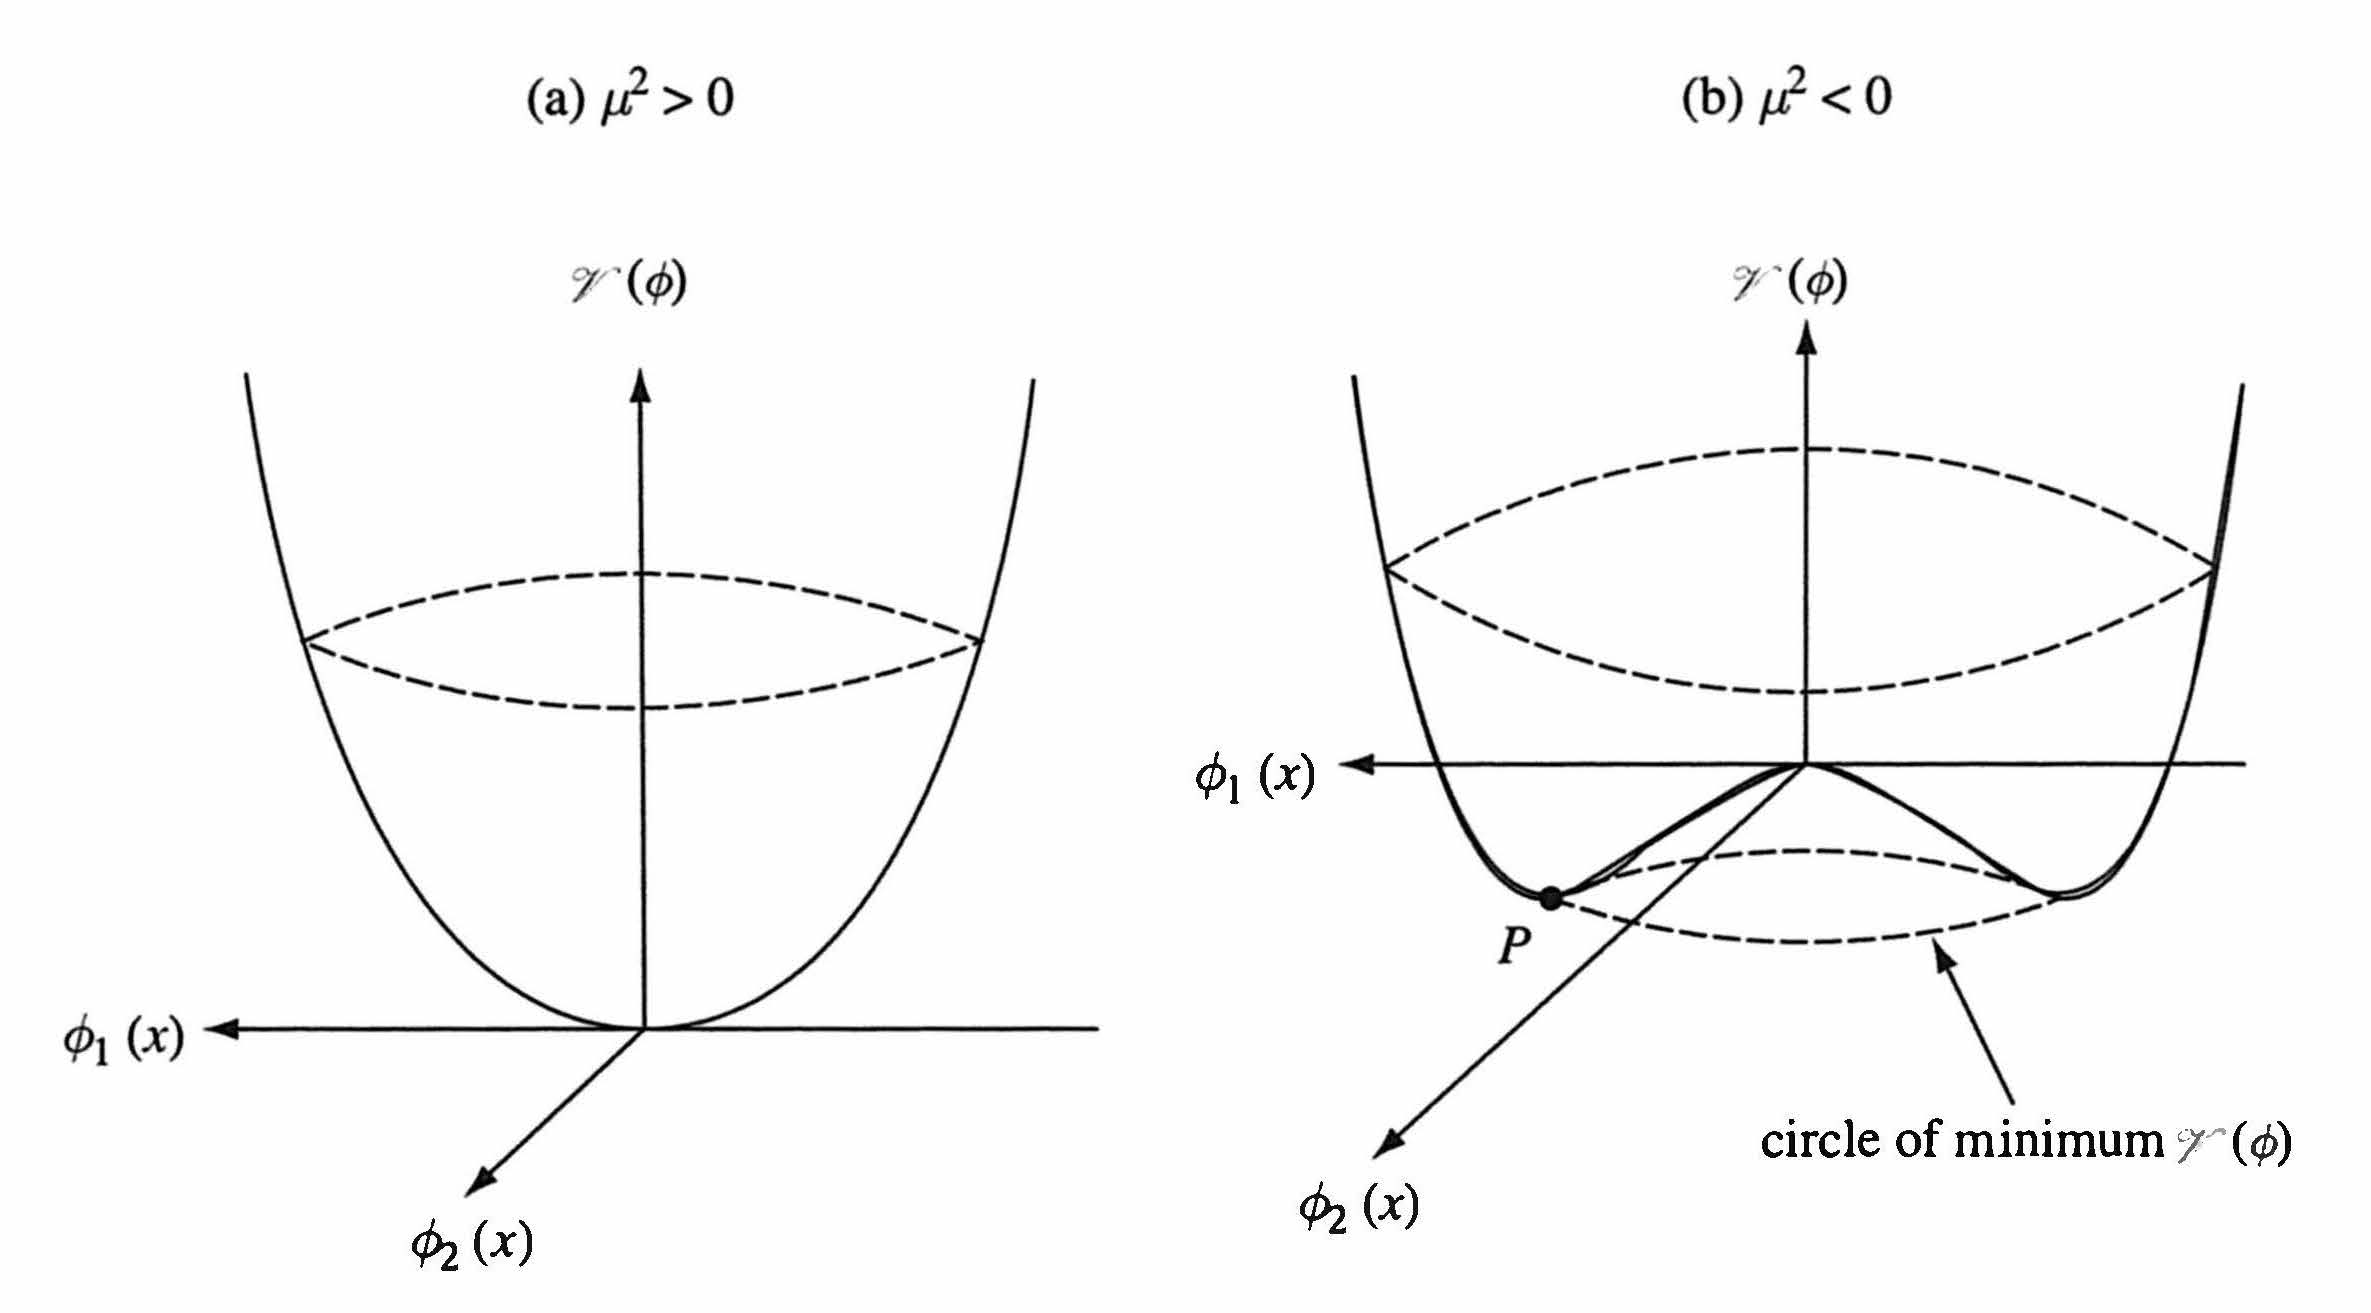
\includegraphics[width=11cm]{img/potential-SSB.jpg}
\caption{Representation of $V(\phi_1^2+\phi_2^2)$ for different signs of $\mu^2$}
\label{fig:SSB-potental}
\end{figure}

\subsection{The minimum of the theory and the choice of the vacuum configuration: the $U(1)$ 
example}

Suppose
\[\phi_0=\frac v{\sqrt2}\qquad v>0\]
Let's redefine our complex field introducing two real fields $\sigma(x)$ and $\pi(x)$:
\[\phi(x)=\frac{\sigma(x)}{\sqrt2}e^{\frac{i\pi(x)}v}\]
then the Lagrangian becomes
\[\mathcal L=\frac12(\partial_\mu\sigma)^2+\frac{\sigma^2}{2v^2}(\partial_\mu\pi)^2-V(\sigma,\pi)\]
where
\[V(\sigma,\pi)=\frac\lambda4(\sigma^2-v^2)^2\]

The first order derivatives of this Lagrangian is given by
\[\begin{cases}
\frac{\partial V}{\partial\sigma}\Big\vert_0=\frac\lambda2\sigma_0(\sigma_0^2-v^2)\vspace{2mm}\\
\frac{\partial V}{\partial\pi}\Big\vert_0=0
\end{cases}\]
hence the vacuum state is given by $\sigma_0=v$ ($\sigma_0=0$ corresponds to negative definite Hessian), no condition over $\pi(x)$ is required.
In order to write explicitly fluctuations about the vacuum state, let's define the field $\tilde \sigma(x)$ as follows
\[\sigma(x)=\tilde\sigma(x)+v\]
in such a way the expected value of $\tilde\sigma(x)$ (i.e. the fluctuation) in the vacuum is $\langle\tilde\sigma\rangle_0=0$
The Lagrangian can be written in terms of fields $\tilde\sigma$ and $\pi$:
\begin{equation}\label{eqn:SSB-lag}\begin{split}
\mathcal L_{\text{SSB}}&=
\frac12(\partial_\mu\tilde\sigma)^2-\frac{(2\lambda v^2)}2\tilde\sigma^2-\lambda v\tilde\sigma^3-\frac\lambda4\tilde\sigma^4+\frac12(\partial_\mu\pi)^2+\p{\frac{2v\tilde\sigma+\tilde\sigma^2}2}(\partial_\mu\pi)^2
\end{split}\end{equation}
This Lagrangian shows kinetic terms for both $\tilde \sigma$ and $\pi$, a massive term only for $\tilde\sigma$:
\[\begin{cases}
m_{\tilde\sigma}^2=2\lambda v^2\\
m_\pi^2=0
\end{cases}\]
Lot of new interactions appears, depending on $\tilde\sigma$ and $\partial_\mu\pi$. Notice that the the fact that $\pi$ has only derivative interactions is a typical consequence of SSB. Anyhow, this is not the most general Lagrangian depending on $\tilde\sigma$ and $\pi$, indeed it depends only on 2 parameters $\lambda$ and $v^2$, and self-interacting couplings 
\[d_3:=\lambda v\qquad\text{and}\qquad d_4:=\frac\lambda4\]
have a relation with the mass of the real scalar field $\tilde\sigma$. 

Notice that eq.~\eqref{eqn:SSB-lag} shows a hidden/residual symmetry called ``shift symmetry'' given by
\[\pi(x)\quad\longrightarrow\quad\pi(x)+\alpha\qquad\text{for}\quad\alpha\in\mathR\]
We can heuristically interpret this symmetry as a redefinition of the field $\phi$ by a phase $e^{i\alpha}$. This is a $U(1)$ symmetry hidden in the SSB, inherited by $\pi$ from the original $U(1)$ symmetry of $\phi$. 



\subsection{The Nambu-Goldstone bosons and the Goldstone theorem}

The example in the previous section is a particular case of a general theorem, the Goldstone theorem, which states that, given a field theory which is Lorentz invariant, local, and has a Hilbert space witha. a positive definite scalar product, if a continuous global simmetry is spontaneously broken, then in the expansion around the symmetry-breaking vacuum there appears a massless particle for each generator that breaks the symmetry. This particle is called a Goldstone (or Nambu-Goldstone) particle. In the previous example the particle was given by the field $\pi(x)$.

The emergence of massless particles corresponds to the possibility of moving, in field space, in the direction of the manifold of vacua. The dimensionality of the manifold of vacua is equal to the number of generators which break the symmetry. In fact, setting the vacuum energy to zero, by definition we have $H\ket0=0$. Since $T^a$ is the generator of a symmetry transformation, it satisfies $[T^a,H]=0$ and therefore
\[H(T^a\ket0)=T^aH\ket0=0\]
So, if $T^a\ket0\neq0$ (and if it is not proportional to $\ket0$ itself) we have found a new state with the minimum energy, i.e. another vacuum state. This is the origin of the fact that we have a Goldstone particle for each generator which breaks the symmetry. 

\subsubsection{Goldstone theorem}

Let's consider a global group of symmetries (compact) $G$, with dimension $d_G$. Let's define a field $\phi$ in the (real) $n$-th dimensional representation of $G$: $\phi=(\phi_1,\dots,\phi_n)^T$. Consider a real Lagrangian for $\phi$:
\[\mathcal L=\frac12(\partial_\mu\phi^T)(\partial^\mu\phi)-V(\phi^T\phi)\]
 with a non-trivial ground state $\langle\phi\rangle_0=\vec v\neq0$, in particular
 \[\frac{\partial V}{\partial\phi_i}\bigg\vert_{\langle\phi_i\rangle=v_i}=0\]
The choice of a vacuum state spontaneously broke down the symmetry group $G$ to a subgroup $H$, that describes the \emph{residual global symmetry}, with $\dim H=d_H$. The vacuum is then invariant under $H$, but not under the remaining elements of $G$, which are denoted as a \emph{coset} and written as $G/H$. The coset is not a subgroup of $G$ (for example, it does not contain the identity element, moreover in general do not have closure property). 

In particular we can consider $N$ generators of $G$, $\{T^a\}=\{X^{\hat a},Y^{\bar a}\}$, where $a=1,\dots,d_G$, $\bar a=1,\dots,d_H$ and $\hat a=1,\dots,d_G-d_H$. The set $\{Y^{\bar a}\}$ is given by the \emph{unbroken generators}
\[Y^{\bar a}\vec v=0\]
and generates the group $H$. Meanwhile, $\{X^{\hat a}\}$ is given by \emph{broken generators}
\[X^{\hat a}\vec v\neq0\]
and generates the coset $G/H$.

For any broken generator corresponds a massless particle in the lagrangian
\[\pi_{\hat a}(x)\qquad\hat a=1,\dots,d_G-d_H\]
and all these massless particles are called \emph{Goldstone bosons}.
\skipline

\noindent
\textit{Proof:}

Consider an infinitesimal transformation of the original symmetry of the Lagrangian 
\[
\phi'=\phi+i\hat\alpha\phi
\qquad\longleftrightarrow\qquad
\phi'_i=\phi_i+i\alpha_aT^a_{ij}\phi_j
\]
Under such a transformation the variation of the potential is zero because of the symmetry of the Lagrangian:
\[\delta V(\phi)=\frac{\partial V}{\partial\phi_i}\delta\phi_i=i\alpha_a\frac{\partial V}{\partial\phi_i}T^a_{ik}\phi_k=0\]
Let's derive with respect to $\phi_j$:
\[i\alpha_a\left\{\frac{\partial^2V}{\partial\phi_i\partial\phi_j}T^a_{ik}\phi_k+\frac{\partial V}{\partial\phi_j}T^a_{ij}\right\}=0\]
And for $\phi=\phi_0$, so that $\langle\phi\rangle_0=\vec v$, the second term in the l.h.s. of the previous equation vanishes since $\phi_0$ is a minimum of $V$ and since the equality must holds for any symmetry transformation (i.e. for each $\hat a$) we obtain
\[\p{\frac{\partial^2V}{\partial\phi_i\partial\phi_j}}_{\langle\phi_i\rangle_0=v_i}T^a_{ik}v_k=0\qquad\forall\,a=1,\dots,d_G\]
I define the mass term $M_{ij}^2$ as the coefficient of the quadratic term in the expansion of $V(\phi)$ about the vacuum state:
\[M_{ij}^2:=\p{\frac{\partial^2V}{\partial\phi_i\partial\phi_j}}_{\langle\phi_i\rangle_0}\]
and
\[w_i^a:=T_{ij}^av_j\]
Then I obtain the following condition:
\[M^2w^a=0\]
hence the matrix $M$ has some zero eigenvalues for some eigenvectors $w^a$.
If we distinguish between eigenvectors of the zero eigenvalue and  other eigenvectors we obtain the distinction between broken and unbroken generators described in the statement of the theorem:
\[W^{\bar a}=Y^{\bar a}v=0\qquad\text{and}\qquad W^{\hat a}=X^{\hat a}v\neq0\]
with $\bar a=1,\dots,d_H$ and $\hat a=1,\dots,d_G-d_H$. Hence $M^2$ has $d_G-d_H$ zero eigenvectors. 

The Goldstone bosons are given by
\[\pi^{\hat a}=i(X^{\hat a}\vec v)\phi=i(X^{\hat a}\vec v)_i\phi_i\]


\begin{example}[$SO(3)\to SO(2)$ SSB]

Take three scalar fields $\phi=(\phi_1,\phi_2,\phi_3)$ in the fundamental representation of $SO(3)$, with the Lagrangian
\[\mathcal L=\frac12(\partial_\mu)^2-V(\phi^\dagger\phi)\]
where
\[V(\phi^\dagger\phi)=\frac\lambda4(\phi^\dagger\phi-v^2)^2\qquad v^2>0\]

The minima condition is given by $\phi^\dagger\phi=v^2$. One possible choice of the vacuum is $\vec v=(0,0,v)$, i.e.
\[\langle\phi_1\rangle_0=\langle\phi_2\rangle_0=0\qquad\langle\phi_3\rangle_v\]

The generators of $SO(3)$ are
\[T_1=\left(\begin{array}{ccc}0 & -i & 0 \\i & 0 & 0 \\0 & 0 & 0\end{array}\right)
\qquad
T_2=\left(\begin{array}{ccc}0 & 0 & -i \\0 & 0 & 0 \\i & 0 & 0\end{array}\right)
\qquad
T_3=\left(\begin{array}{ccc}0 & 0 & 0 \\0 & 0 & -i \\0 & i & 0\end{array}\right)
\]
in particular $T_1$ is the unbroken generator, while $T_2$ and $T_3$ are the broken generators:
\[T_1\vec v=0\qquad T_2\vec v\neq0\qquad T_3\vec v\neq0\]

Physical fields are the ones that in the vacuum state has zero expectation value, and by defining
\[\phi_3=\tilde\phi_3+v\]
we obtain that physical fields are $\phi_1$, $\phi_2$ and $\tilde\phi_3$. 

The Goldstone bosons are
\[\pi_1=\frac iv(T_2\vec v)\phi=\phi_1\qquad \pi_2=\frac iv(T_3\vec v)\phi=\phi_2\]
which are massless fields, while expanding the Lagrangian in terms of physical fields we obtain that the mass of the particle described by $\tilde\phi_3$ is $m_3^2=2\lambda v$. 


\end{example}

Another example of SSB is given by the spontaneous symmetry breaking of $SU(2)\times SU(2)$, whose Goldstone bosons are the pions. 

\section{Spontaneous Symmetry Breaking of a local symmetry}
\textsf{Schwartz sec. 28.3-28.4; Peskin sec. 20.1, 21.1; Mandl sec. 18.2; Halzen sec. 14.8-14.9}\\

What happens if we include both local gauge invariance and spontaneous symmetry breaking in the same theory? In this section we will find that this combination of ingredients leads to new possibilities for the construction of quantum field theory models. We will see that spontaneous symmetry breaking requires gauge vector bosons to acquire mass. However, the interactions of these massive bosons are still constrained by the underlying gauge symmetry, and these constraints can have observable consequences. 

In elementary particle physics, the principal application of spontaneously broken local symmetry is in the currently accepted model of weak interactions. We will see that it makes a number of precise and successful predictions for weak interactions phenomena. Remarkably, this model also unifies the weak interactions with electromagnetism in a single larger gauge theory. 

\subsection{$U(1)$ gauge theory minimally coupled to a complex scalar field with a non-trivial scalar potential}

As our first example, consider a complex scalar field couple both to itself and to an electromagnetic field:
\[\mathcal L=-\frac14F_{\mu\nu}F^{\mu\nu}+(D_\mu\phi)^\dagger(D^\mu\phi)-V(\phi^\dagger\phi)\]
with $D_\mu=\partial_\mu+igA_\mu$. This Lagrangian is invariant under the local $U(1)$ transformation
\[\phi(x)\,\to\,e^{ig\alpha(x)}\phi(x)\hspace{1.5cm}A_\mu(x)\,\to\,A_{\mu}-\partial_\mu\alpha(x)\]
which implies
\[(D_\mu\phi)\,\to\,e^{ig\alpha(x)}(D_\mu\phi)\]
If we choose the potential in $\mathcal L$ to be of the form
\[V(\phi^\dagger\phi)=\lambda\p{\phi^\dagger\phi-\frac{v^2}2}^2\]
with $v^2>0$, the field $\phi$ will acquire a vacuum expectation value and the $U(1)$ global symmetry will be spontaneously broken. 

\subsection{The minimum of the theory and the choice of the vacuum configuration}

Let us consider the requirements for the vacuum configurations. The Hamiltonian for this theory is 
\[\mathcal H=\int\de^3x\left\{\frac12(F_{0i})^2+\frac14(F_{ij})^2+(D_0\phi)^\dagger(D_0\phi)+(D_i\phi)^\dagger(D_i\phi)+V(\phi^\dagger\phi)\right\}>E_{\text{min}}\]
hence the vacuum configuration must satisfy the followings:
\begin{enumerate}[label=(\arabic*)]
\item $A^\mu$ is a pure gauge configuration $A^0_\mu=\partial_\mu\alpha(x)$, this implies $F_{0i}=F_{ij}=0$
\item $\phi_0$ is a constant field configuration: $(D_\mu\phi_0)=0$, this is satisfied by taking $\phi_0=\frac c{\sqrt2}e^{ig\alpha}$ for some constant $c$ and $0\leq\alpha<2\pi$
\item $V(\phi_0^\dagger\phi_0)$ is a minimum for $V$, hence $\phi_0^*\phi_0=\frac{v^2}2$
\end{enumerate}
If we choose $\alpha(x)=0$ we obtain the vacuum state
\[\langle A_\mu\rangle_0=A^0_\mu=0\hspace{1.5cm}\langle\phi\rangle_0=\phi_0=\frac v{\sqrt2}\]
Let's define fluctuations about the vacuum configuration:
\[\phi(x)=\frac{v+\tilde\sigma}{\sqrt2}e^{i\pi(x)/v}\qquad\to\qquad\langle\sigma\rangle_0=v\qquad\langle\tilde\sigma\rangle_0=0\]
In terms of $\tilde\sigma$ and $\pi$ the Lagrangian density becomes
\begin{equation}\label{eqn:SSB-gauge-pi}\begin{split}
\mathcal L_{\text{SSB}}
&=-\frac14F_{\mu\nu}F^{\mu\nu}+\frac{g^2}2(v+\tilde\sigma)^2\p{A_\mu+\frac1{gv}\partial_\mu\pi}^2\\
&\quad+\frac12(\partial_\mu\tilde\sigma)(\partial^\mu\tilde\sigma)-\frac12m_{\tilde\sigma}^2\tilde\sigma^2-\frac\lambda4(4v\tilde\sigma^3+\tilde\sigma^4)
\end{split}\end{equation}
where $m_{\tilde\sigma}^2=2\lambda v^2$ is the mass term for $\tilde\sigma$ field. 

\subsection{The Would Be Goldstone Boson (WBGB) and the longitudinal vector boson d.o.f.}

The direct interpretation of eq.~\eqref{eqn:SSB-gauge-pi} leads to difficulties. It contains the equation for a real Klein-Gordon field with mass $\sqrt{2\lambda v^2}$. However, the mixed term $A^\mu\partial_\mu\pi$ shows that $A^\mu$ and $\pi$ are not independent normal coordinates, and one cannot interpret $A_\mu$ and $\pi$ as massive vector bosons and a massless scalar boson respectively. This difficulty also shoes up if we count degrees of freedom: two from the complex scalar field $\phi$ and two from the real massless vector field $A^\mu$ (i.e. for massless photons there are only two independent polarization states, the third is eliminated by gauge invariance). In $\mathcal L_{\text{SSB}}$ the real scalar fields $\tilde\sigma$ and $\pi$ each represent one degree and the real massive vector field $A^\mu$ contributes three degrees (corresponding to three independent polarization states), i.e. the SSB Lagrangian appears to have five degrees of freedom. Of course, a change of variables cannot alter the number of degrees of freedom of a system. We most conclude that the Lagrangian density contains an unphysical field which does not represent real particles and which can be eliminated. 

The field $\pi$ can be eliminated through an appropriate choice of a gauge, in particular we can define the following boson vector field:
\[B_\mu:=A_\mu+\frac1{gv}(\partial_\mu\pi)\hspace{1.5cm}B_{\mu\nu}:=\partial_\mu B_\nu-\partial_\nu B_\mu\]
and introducing this field in the Lagrangian we obtain
\begin{equation}\label{eqn:SSB-gauge}\begin{split}
\mathcal L_{\text{SSB}}
&=-\frac14B_{\mu\nu}B^{\mu\nu}+\frac12m_B^2B^\mu B_\mu+\frac{g^2}2(2v\tilde\sigma+\tilde\sigma^2)B^\mu B_\mu\\
&\quad+\frac12(\partial_\mu\tilde\sigma)(\partial^\mu\tilde\sigma)-\frac12m_{\tilde\sigma}^2\tilde\sigma^2-\frac\lambda4(4v\tilde\sigma^3+\tilde\sigma^4)
\end{split}\end{equation}
where we introduce the mass term for the $B^\mu$ field $m_B^2:=g^2v^2$. Hence the SSB of a gauge theory leads to the introduction to a massive vector boson, which ``eats'' the Goldstone boson $\pi$ and the initial massless gauge field $A^\mu$. The the theory of SSB for gauge theories the field $\pi$ is called \emph{Would Be Goldstone Boson (WBGB)}.

By giving a mass to $A_\mu$ introducing $B_\mu$, we have clearly introduced a longitudinal polarization for the gauge field. 

\subsection{The Higgs mechanism}

What we obtained is a remarkable result. Having started from a complex scalar field and a massless real vector field, we have ended up with the Lagrangian density for a real scalar field and a massive real vector field. The number of degrees of freedom is four in both cases. Of the two degrees of freedom of the comple field $\phi$, one has be taken up by the vector field $A_\mu$, which as become massive ($B_\mu$) in the process; the other shows up as the real field $\tilde\sigma$. 

This phenomenon by which a vector boson acquires mass without destroying the gauge invariance of the Lagrangian density is known as the \emph{Higgs mechanism}, and the massive spin-0 boson associated with the field $\tilde\sigma$ is called a Higgs boson or a Higgs scalar. The Higgs mechanism does not generate Goldstone bosons, in contrast to the spontaneous symmetry breaking of the global phase invariance of the Goldstone model. In essence, the field $\pi$ which in the Goldstone model was associated with the massless Goldstone boson, has been eliminated by gauge invariance, and the degree of freedom of $\pi$ has been transferred to the vector field $B_\mu$. 

\subsection{Feynman rules in the Unitary gauge and in the $R_\xi$ gauge}

We notice that eq.~\eqref{eqn:SSB-gauge-pi} still exhibits a local $U(1)$ symmetry:
\[\tilde\sigma(x)\,\to\,\tilde\sigma(x)\hspace{1.5cm}\pi(x)\,\to\,\pi(x)+gv\alpha(x)\hspace{1.5cm}A_\mu(x)\,\to\,A_\mu(x)-\partial_\mu\alpha(x)\]
even though in this case I have a mass term in the boson part of the Lagrangian. This is a consequence of the original gauge symmetry of the Lagrangian. Moreover, notice that $\tilde\sigma$ is invariant under this transformation, so it is a singlet under $U(1)$. 

The field $B_\mu$ is a specific gauge choice for such a symmetry, called \emph{unitary gauge}. In the unitary gauge the Lagrangian of a SSB theory shows explicitly the physical fields. 

In some cases, especially if we want to quantize such a theory, we may use different gauge choices, introducing (non-unitary) gauge fixing terms in the Lagrangian, which corresponds to non-physical d.o.f. of the theory (e.g. the longitudinal polarization for the Maxwell field). In particular, the so called \emph{$R_\xi$ gauge choice} corresponds to the introduction of the following gauge fixing term in eq.~\eqref{eqn:SSB-gauge-pi}:
\begin{equation}\label{eqn:SSB-gauge-Rxi}
\mathcal L_{\text{GF}}:=-\frac1{2\xi}(\partial_\mu A^\mu-\xi(gv)\pi)^2=-\frac1{2\xi}(\partial_\mu A^\mu)^2-\frac12(\xi g^2v^2)\pi^2+gv(\partial_\mu A^\mu)\pi
\end{equation}
which corresponds to the introduction of a mass term $m_\pi^2=\xi^2g^2v^2=\xi^2m_B^2$ for the field $\pi$ and a cross mixing term $(\partial_\mu A^\mu)\pi=-A^\mu(\partial_\mu\pi)+\partial_\mu(A^\mu\pi)$ which cancels the mixing term in eq.~\eqref{eqn:SSB-gauge-pi}. 

If we consider the full Lagrangian with $R_\xi$ gauge fixing term $\mathcal L=\eqref{eqn:SSB-gauge-pi}+\eqref{eqn:SSB-gauge-Rxi}$ we can quantize the SSB theory and obtain following Feynman rules ($M_A^2=g^2v^2$):

\begin{subequations}\begin{alignat}{3}
A_\mu:&&\qquad
\begin{tikzpicture}[baseline=(a)]
	\begin{feynman}
		\vertex[label={[yshift=0.1cm, font=\footnotesize]$\mu$}](a);
		\vertex[right=2cm of a, label={[yshift=0.1cm, font=\footnotesize]$\nu$}](b);
		\diagram*{
			(a)--[boson, momentum={[arrow shorten=0.3, font=\footnotesize]$k$}](b)
		};
	\end{feynman}
\end{tikzpicture}
\qquad&&D^A_{\mu\nu}(k)&=
-\frac i{k^2-M_A^2}\p{\eta_{\mu\nu}-(1-\xi)\frac{k_\mu k_\nu}{k^2-\xi M_A^2}}\\
%
\tilde\sigma:&&\qquad
\begin{tikzpicture}[baseline=(a)]
	\begin{feynman}
		\vertex[label={[yshift=0.1cm, font=\footnotesize]$\hspace{1mm}$}](a);
		\vertex[right=2cm of a, label={[yshift=0.1cm, font=\footnotesize]$\hspace{2mm}$}](b);
		\diagram*{
			(a)--[scalar, momentum={[arrow shorten=0.3, font=\footnotesize]$k$}](b)
		};
	\end{feynman}
\end{tikzpicture}
\qquad&&D^{\tilde\sigma}(k)&=
-\frac i{k^2-m_{\tilde\sigma}^2}\\
%
\pi:&&\qquad
\begin{tikzpicture}[baseline=(a)]
	\begin{feynman}
		\vertex[label={[yshift=0.1cm, font=\footnotesize]$\hspace{1mm}$}](a);
		\vertex[right=2cm of a, label={[yshift=0.1cm, font=\footnotesize]$\hspace{2mm}$}](b);
		\diagram*{
			(a)--[ghost, momentum={[arrow shorten=0.3, font=\footnotesize]$k$}](b)
		};
	\end{feynman}
\end{tikzpicture}
\qquad&&D^{\pi}(k)&=
-\frac i{k^2-\xi M_A^2}
\end{alignat}\end{subequations}

Notice that for $\xi\to\infty$ I obtain the unitary gauge eq.~\eqref{eqn:SSB-gauge}, in this case the propagator for the gauge field becomes ($A_\mu=B_\mu$)
\[D^B_{\mu\nu}(k)=-\frac i{k^2-M_B^2}\p{\eta_{\mu\nu}-\frac{k_\mu k_\nu}{M_B^2}}\]
so we obtain (as we expected) the propagator of a Proca field, i.e. a massive vector propagator. Moreover, for $\xi\to\infty$ we have $D^\pi=0$, and the non-physical Goldstone boson disappear from Feynman diagrams. 

As we had disclosed, the gauge $R_\xi$ it is useful to describe the renormalization of SSB gauge theories. Indeed, for $k\to\infty$ the degree of divergence of $D^A_{\mu\nu}(k)$ is the same as the one of the photon propagator in QED:
\[D^A_{\mu\nu}(k)=-\frac i{k^2-M_A^2}\p{\eta_{\mu\nu}-(1-\xi)\frac{k_\mu k_\nu}{k^2-\xi M_A^2}}
\approx -\frac i{k^2}\p{\eta_{\mu\nu}-(1-\xi)\frac{k_\mu k_\nu}{k^2}}\]
Since the renormalizability does not depend on the gauge choice, SSB gauge theories are renormalizable. 

\subsection{Generalization of the Higgs mechanism to generic (compact) group}

In this section we discuss the SSB of a generic gauge theory. For definiteness we consider the case $G=SU(N)$, but the following derivation holds in general. Consider a complex scalar field $\phi$ in the $N$-dimensional fundamental representation of $G$. Suppose that the Lagrangian shows a potential with a non-trivial minimum condition in the form $V(\phi^\dagger\phi)=\lambda(\phi^\dagger\phi-\frac{\vec v^2}2)^2$ and take as vacuum state $\langle\phi\rangle_0=\phi_0=(0,\dots,v_i,\dots,0)$ for some $v_i\neq0$. 

The choice of a vacuum state will broke doen the symmetry group $G$ to a subgroup $H$. As we seen in general, $d_H$ generators $\{Y^{\bar a}\}$ of $G$ are unbroken, while $d_G-d_H$ generators $\{X^{\hat a}\}$ will be broken by the choice of a vacuum state. 

Consider the minimal coupling of the Lagrangian:
\[(D_\mu\phi)^\dagger(D^\mu\phi)=[(\partial_\mu+ig\hat A_\mu)\phi]^\dagger[(\partial^\mu+ig\hat A^\mu)\phi]\]
If we define the fluctuation $\tilde\phi$ as $\phi=\tilde\phi-\vec v$ we can express the previous component of the Lagrangian in terms of this field, obtaining
\[(D_\mu\tilde\phi)^\dagger(D^\mu\tilde\phi)-ig\left\{(\partial^\mu\tilde\phi)^\dagger\hat A_\mu(\vec v+\tilde\phi)-(\vec v+\tilde\phi)^\dagger A^\mu(\partial_\mu\tilde\phi)\right\}+g^2(\vec v+\tilde\phi)^\dagger\hat A^\mu\hat A_\mu(\vec v+\tilde\phi)\]
so I obtained a mass term for gauge bosons:
\[g^2\vec v^\dagger\hat A^\mu\hat A_\mu\vec v=g^2A_a^\mu A_\mu^b\underbrace{(T^a\vec v)^\dagger(T^b\vec v)}_{(M_B^2)_{ab}}\]
The matrix $M_B^2$ is positive definite and has exactly $d_G-d_H$ non-zero eigenvalues due to $(X^{\hat a}\vec v)\neq0$ and $( Y^{\bar a}\vec v)=0$. 














\end{document}